\documentclass[11pt]{article}

\usepackage[utf8]{inputenc}
\usepackage[portuguese]{babel}
\usepackage{indentfirst}
\usepackage{natbib}
\usepackage{graphicx}
\usepackage{adjustbox}
\usepackage{float}
\usepackage{geometry}
 \geometry{
    a4paper,
    total={130mm,227mm},
    left=30mm,
    right=30mm,
    top=20mm,
    bottom=20mm
}
\setlength\abovecaptionskip{-2pt}
 
\renewcommand{\contentsname}{Índice}

\begin{document}

\begin{titlepage}
    \begin{center}
        
\includegraphics[width=0.3\textwidth]{images/capa/EscolaEngenhariaUM.jpeg}
    
        \vspace{1cm}
        
        \textbf{\LARGE Comunicações por Computador}
    
        \vspace{0.5cm}
        \textbf{\Large Trabalho Prático 2}

        \vspace{1.3cm}
        
        \textbf{\large Luís Pedro Oliveira de Castro Vieira A89601 \\
        José Pedro de Castro Ferreira A89572 \\
        Luís Enes Sousa A89597}

        \vspace{1.5cm}
        \begin{figure}[hbt!]
            \minipage{0.32\textwidth}
                \frame{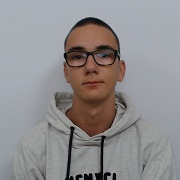
\includegraphics[width=\linewidth]{images/capa/massini.jpg}}
                \centering
                \captionsetup{A89601}
            \endminipage\hfill
            \minipage{0.32\textwidth}
                \frame{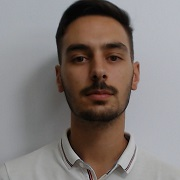
\includegraphics[width=\linewidth]{images/capa/8free.jpg}}
                \centering
                \captionsetup{A89572}
            \endminipage\hfill
            \minipage{0.32\textwidth}
                \frame{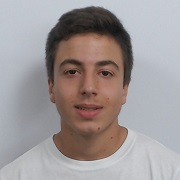
\includegraphics[width=\linewidth]{images/capa/80.jpeg}}
                \centering
                \captionsetup{A89597}
            \endminipage
        \end{figure}
        
       \vspace{8cm}
        
        25 de maio de 2021
        
    \end{center}
\end{titlepage}

\tableofcontents
\thispagestyle{empty}
\cleardoublepage

\setcounter{page}{1}

\section{Introdução}

\par No âmbito da Unidade Curricular de Comunicações por Computador, foi proposto ao grupo que implementasse um serviço de transferência de ficheiros, baseado na utilização do protoloco TCP e também na manipulação e exploração do protocolo UDP.\\

\par Assim sendo, o objetivo deste trabalho é implementar um \textit{gateway} de aplicação, designado por HttpGw, que opere exclusivamente com o protocolo HTTP/1.1
e que seja capaz de responder a múltiplos pedidos em simultâneo, recorrendo a a uma pool dinâmica de servidores de alto desempenho, designados por FastFileSrv, e usando um protocolo a especificar para o efeito, FS Chunk Protocol.


%-----------------------------------------------------------------%
\section{Arquitetura da Solução}

De forma a cumprir os requisitos do enunciado deste trabalho prático, começamos por estabelecer as ligações entre cliente, HttpGw e FastFileSrv.

Primeiramente, estabelecemos a ligação TCP entre cliente e HttpGw, criando uma \textit{Thread} no HttpGw que fica à escuta na porta TCP 8080.\\

De seguida, definimos a ligação entre FastFileSrv e o HttpGw. Para tal, o HttpGw cria um \textit{Socket} UDP na porta 8888, pelo qual os diferentes FastFileSrv's vão comunicar.

Depois, foi necessário definir uma entidade para processar um pedido do cliente, pedir os ficheiros necessários e devolvê-los ao cliente. Para tal, criamos a classe HttpGwWorker.\\

Entretanto, decidimos implementar o nosso protocolo na comunicação UDP. Para tal, incapsulamos a nossa classe \textit{Packet} num \textit{DatagramPacket}, que será enviado no \textit{Socket}.

Foi, também, necessário definir um procedimento que permitisse controlar a inatividade de um FastFileSrv. Desta forma, os FastFileSrv's ligados ao HttpGw, enviam um pacote \textit{Beacon} periodicamente para o HttpGw.


\begin{figure}[H]
    \centering
    \frame{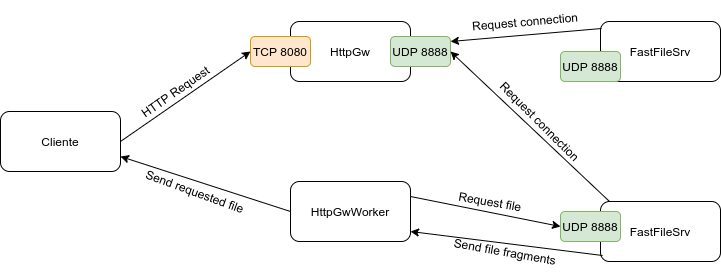
\includegraphics[width=1\textwidth]{images/Untitled Diagram.png}}
    \caption{Arquitetura da solução}
\end{figure}


%-----------------------------------------------------------------%
\newpage
\section{Especificação do Protocolo}

\par Durante o desenho do protocolo que o grupo iria implementar esteve sempre a ser considerado aquilo que facilitaria e tornaria o nossos sistema, num sistema fiável, funcional e capaz no trabalho que precisava de desempenhar.

\par Tivemos também em conta aquilo que o protocolo sobre o qual o iríamos implementar nos seria capaz de fornecer uma vez que já existe.  Tudo com a visão de cumprir com os requisitos obrigatórios, e mais, de forma a podermos explorar as nossas capacidades e conhecimento.

\subsection{Formato das Mensagens Protocolares}

\par Assim o nosso pacote contém informação que achamos efetivamente necessária adicionalmente à que o pacote do protocolo UDP já acarreta, sendo tais:

\begin{table}[!h]
\centering
\begin{tabular}{|c|}
\hline
\textbf{Pacote}                                                            \\ \hline
Identificador do Pacote                                                    \\ \hline
Tipo do Pacote                                                             \\ \hline
Offset do Pacote - para casos de pacotes fragmentos                        \\ \hline
\multicolumn{1}{|l|}{Quantidade de fragmentos totais de uma transferência} \\ \hline
Payload                                                                    \\ \hline
\end{tabular}
\end{table}

\par Para o nosso pacote estimamos um total de 5016 bytes em uso: 4 bytes para o identificador, 4 para o tipo do pacote, 4 para o offset, 4 para o total de fragmentos de uma dada transferência e 4096 bytes para o payload.\\

\par A designação de 4096 bytes foi debatida entre o grupo por vários motivos mas o principal foco no contexto do trabalho é, sem dúvida, a fragmentação.\\

\par Os pacotes enviados em UDP são capazes de suportar até 65 535 bytes, o que facilitaria bastante no envio de ficheiros de maiores dimnesões. No entanto como o UDP se trata de um protocolo não orientado à conexão e sem controlos de erros exímios, utilizar um tamanho tão grande para o payload poderia trazer grandes dificuldades ao nosso programa, uma vez que cada transferência pedida pelo cliente era muito mais suscetível de não ser efetivamente realizada.\\

\par Assim, achamos que 4096 bytes é o tamanho ideal para que, mesmo levando a fragmentação, seja minimizado o risco de perdas de pacotes no meio das transferências de ficheiros.

\subsubsection{Tipos do Pacote}

\par Ao definirmos a PDU a utilizar definimos 4 tipos de pacotes a serem enviados:

\begin{table}[!h]
\resizebox{\textwidth}{!}{
\begin{tabular}{|c|c|}
\hline
\textbf{Tipo} & \textbf{Significado}                                   \\ \hline
BEACON          & Informa que o servidor ainda se encontra a comunicar com o \textit{gateway} HttpGW \\ \hline
CONNECTION    & Pedido de ligação por parte do FastFileSrv ao \textit{gateway}  \\ \hline
ACK\_CONNECTION & Resposta por parte do \textit{gateway} a confirmar a conexão do FastFileSrv        \\ \hline
DATA          & Informa que o pacote contém dados do pedido do cliente \\ \hline
\end{tabular}
}
\end{table}

\par Os pacotes do tipo \textit{\textbf{BEACON}} servem como avisos ao \textit{gateway} de que o servidor que os está a enviar, ainda se encontra conectado ao mesmo e que portanto não o deve descartar. Quando um servidor deixa de enviar estes pacotes após um dado tempo, o \textit{gateway} considera, por motivos de segurança, que o servidor já não é viável e portanto remove-o da pool de servidores conectados a si, até uma conexão posterior nova.\\

\par Já os pacotes do tipo \textit{\textbf{CONNECTION}}, são os pacotes enviados no início aquando da requisição de conexão por parte do FastFileSrv ao HttpGw para se registar na sua base de dados e poder participar ativamente nos pedidos feitos pelo utilizador.\\

\par A este pedido é enviado o pacote de resposta do tipo ACK\_Connection por parte do HttpGw a aceitar e confirmar a conexão do FastFileSrv que tinha enviado previamente o pacote do tipo \textit{\textbf{CONNECTION}}.\\

\par Por fim, os pacotes do tipo \textit{\textbf{DATA}} são os pacotes enviados pelos FastFileSrv que contém a informação do ficheiro pedido pelo cliente aquando do pedido HTTP GET captado pelo \textit{gateway}.\\

\subsection{Controlo de Erros}

\par Um ponto fulcral no qual infelizmente falhamos por incapacidade de implementação é o controlo de erros. Qualquer conexão está sujeita aos mesmos e portanto deveríamos ter sido capazes de efetuar com sucesso o controlo de erros para garantir a integridade da transferência. O objetivo a ser implementado para o controlo de erros seria a retransmissão de informação e o checksum, embora não tenhamos sido capazes de concretizar nenhum dos dois.

\par No caso da retransmissão de pacotes, deveríamos ter introduzido um novo tipo de pacote que serviria como uma espécie de ACK que o UDPListener lançaria cada vez que recebesse um pacote fragmentado de um ficheiro. Caso o FastFileSrv não recebesse essa confirmação para um dado pacote trataria de re-enviar o mesmo de modo a que o cliente recebesse o ficheiro sem qualquer problemas.\\

\par Quando ao controlo através do checksum, seria necessário calcular uma chave, podendo basearmo-nos naquilo que é feito no protocolo TCP, e enviar juntamente com o pacote para posterior confirmação do mesmo.

\subsection{Múltiplos Servidores}

\par Uma outra funcionalidade mencionada no enunciado é a capacidade de para um pedido de um cliente, requisitar a vários servidores o mesmo ficheiro de modo a tornar mais eficiente a transferência.\\ 

\par O objetivo seria para cada ficheiro pedido pelo cliente, atribuir a cada servidor uma secção do mesmo que ele depois enviaria ao cliente. Isto diminuiria não só o tempo de download como a probabilidade de falhas nas transferências.


\subsection{Interações}

\par Em todo o nosso programa existem diversas interações que refletem o bom funcionamento do mesmo, no entanto iremos apenas apresentar e enunciar algumas das que considerámos serem mais importantes, as que mais representam o que a aplicação em si é supostos realizar.

\subsubsection{Pedido de Conexão ao \textit{Gateway} por parte do \textit{FastFileSrv}}

\par Quando um servidor \textit{FastFileSrv} se pretende conectar ao \textit{gateway} indica como argumentos o endereço e a porta do mesmo, enviando um pedido de conexão com um pacote do tipo \textit{CONNECTION}. Ao receber este pacote o \textit{gateway} apercebe-se que existe um servidor a tentar conectar-se e caso a ligação seja válida, isto é, caso já não exista um outro servidor com o mesmo endereço, envia ao servidor uma resposta do tipo \textit{ACK\_CONNECTION}.\\

\par Por sua vez, quando o servidor recebete este pacote, sabe que a ligação foi aceite e começa por sua vez a enviar pacotes do tipo \textit{BEACON} continuamente, como forma de sinaliza ao \textit{HttpGw} que se encontra ativo e pronto a receber pedidos de clientes.\\

\par Quando um servidor é fechado, como deixa de enviar pacotes \textit{BEACON}, o \textit{gateway} irá removê-lo da pool de servidores ativos como uma medida de segurança, terminando a ligação com os mesmos.

\begin{figure}[!ht]
    \centering
    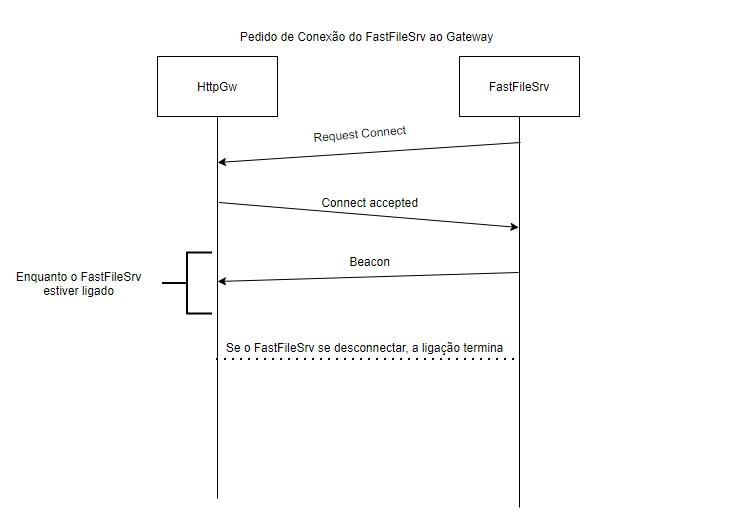
\includegraphics[scale=0.8]{images/RequestUDPconnection.jpg}
    \caption{Pedido de Conexão do FastFileSrv ao HttpGw}
    \label{fig:connect}
\end{figure}

\subsubsection{Pedido HTTP Get do Cliente}

\par O \textit{HttpGw} tem constantemente um socket \textit{TCP} à escuta por pedidos dos clientes na porta 8080 (não é usada a porta 80 uma vez que esta se encontra reservada por certos protocolos e seria necessário permissões de root para sobrepôr).\\

\par Quando um cliente efetua um comando \textit{wget http://endereço\_gateway:port\_gateway/nome\_do\_ficheiro} este socket vai receber o pedido e vai reencaminhá-lo para um servidor \textit{FastFileSrv}.\\

\par Os FastFileSrv começam então o processo de obtenção do ficheiro e juntam a informação toda sobre o mesmo numa thread que se encontra constantemente a correr no HttpGw por cada cliente conectado ao mesmo. Essa thread, denominada HttpGwWorker, está responsável por juntar os pacotes do tipo \textit{DATA} enviados pelos FastFileSrv para o UDPListener, e efetivamente enviar para o cliente o ficheiro pedido.\\

\par Caso o ficheiro seja demasiado grande para o tamanho máximo de pacote por nós estipulado, então ocorrerá a fragmentação do ficheiro a ser enviado ao cliente. Quando isto acontece, o HttpGwWorker espera que o UDPListener tenha recebido todos os fragmentos do ficheiro e depois junta os mesmos para enviar ao cliente, na ordem em que é supostos eles serem enviados, graças ao offset presente no cabeçalho do nosso pacote.


\begin{figure}[!ht]
    \centering
    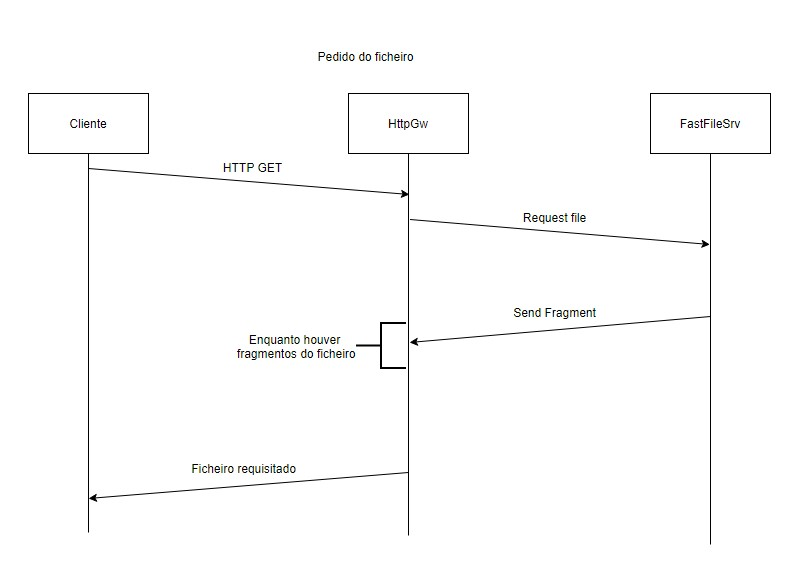
\includegraphics[scale=0.8]{images/FileRequest.jpg}
    \caption{Pedido HTTP Get do Cliente}
    \label{fig:request}
\end{figure}


%-----------------------------------------------------------------%
\cleardoublepage
\section{Implementação}

Em relação à implementação do nosso projeto, este pode-se dividir em duas partes principais: o \textbf{HttpGw} (\textit{Gateway}) e os \textbf{FastFileSrv}'s.

\subsection{HttpGw}

Neste package encontramos as classes referentes ao \textit{Gateway}, que controlam o tráfego entre os clientes e os servidores.

\subsubsection{HttpGw.java}

Esta é a classe principal do \textit{Gateway}, que cria os \textit{Sockets} para comunicações, tanto TCP como UDP, e que lança \textit{Threads} para escutar nesses \textit{Sockets}. Também é responsável pela criação da \textit{Thread} que interpreta os pacotes \textit{Beacon} recebidos dos servidores.

\subsubsection{TCPListener.java}

Esta classe é responsável por escutar os pedidos HTTP dos clientes na porta TCP 8080. Quando chega um pedido a essa porta, é criada uma \textit{Thread} para o processar e enviar o seu resultado ao cliente.


\subsubsection{UDPListener.java}

Esta classe é responsável por todas as comunicações que chegam ao \textit{Gateway} e vindas de um servidor. Estas podem ser um pedido de conexão, um pacote \textit{Beacon} ou um pacote de dados. Durante a sua execução, esta está à escuta na porta UDP 8888. Quando recebe um pacote, começa por perceber de onde vem e analisar o seu tipo.

Caso receba um pedido de conexão, verifica se esse servidor já se encontra conectado. Caso contrário, adiciona-o aos servidores conectados e envia um pacote de confirmaçao de conexão.

Caso receba um pacote \textit{Beacon}, envia este para o \textit{Beacon Handler}, que processa a sua informação.

Caso receba um pacote de dados, envia-o para o \textit{HttpGwWorker} correspondente.

\subsubsection{BeaconHandler.java}

Esta classe é responsável por controlar o tempo de inatividade dos servidores. Durante a sua execução, esta atualiza o tempo de inatividade de todos os servidores conectados. Caso algum servidor fique inativo
durante um tempo superior a um tempo máximo definido, este é removido do \textit{Gateway}.

Esta classe é, ainda, responsável pelo processamento de todos os pacotes \textit{Beacon} recebidos pelo \textit{Gateway}. Este processamento consiste em analizar o endereço do pacote e \textit{resetar} o tempo de inatividade do servidor associado.

\subsubsection{HttpGwWorker.java}

Esta classe é responsável por analisar o pedido de um cliente e retribuir o ficheiro correspondente. Para tal, esta começa por processar o cabeçalho HTTP recebido na conexão TCP. Posto isto, estabelece conexão com um \textit{FastFileSrv} disponível, enviando o pedido do ficheiro. Depois, espera que todos os fragmentos sejam enviados. Caso o pacote não tenha sido fragmentado, os dados são enviados diretamente para o cliente. Caso contrário, o \textit{HttpGwWorker} trata de desfragmentar os pacotes, procedendo, então, ao seu envio para o cliente.

\subsubsection{FastFileSrvInfo.java}

Esta classe guarda informações sobre um servidor, como a porta à qual está conectado, o tempo de inatividade e a sua disponibilidade.


\subsection{FastFileSrv}

Neste package encontramos as classes referentes aos servidores, que assumem o envio dos ficheiros requisitados pelos clientes.

\subsubsection{FastFileSrv.java}

Esta classe representa a classe principal de um servidor. Quando executada, começa por estabelecer a conexão com o \textit{Gateway}. Depois, cria uma \textit{Thread} para enviar pacotes \textit{Beacon} e fica à espera de um pedido de um cliente, vindo de um \textit{HttpGwWorker}.

Quando chega um pacote, este processa a sua informação, obtendo o nome do ficheiro requisitado. Posto isto, lê o conteúdo do ficheiro e encapsula-o num pacote para este ser enviado pelo protocolo UDP. Caso o tamanho do ficheiro seja maior que o máximo de dados de um pacote, o \textit{FastFileSrv} terá de fragmentar a informação, enviando-a em diversos pacotes, devidamente identificados.

\subsubsection{FastFileSrvBeacon.java}

Esta classe é responsável por enviar os pacotes \textit{Beacon} para o \textit{Gateway}, de forma a informar que o servidor está ativo.

\subsection{FS Chunk Protocol}

\subsubsection{Packet.java}

Esta classe representa a nossa implementação do \textit{FS Chunk Protocol}. Desta forma somos capazes de fragmentar as nossas mensagens, devido à presença dos campos: \textit{id}, \textit{offset} e \textit{fragments}. Ainda somos capazes de identificar o tipo do pacote, através do campo \textit{type}. Este pacote tem, ainda, um campo \textit{data}, que permite tranferir qualquer informação no protocolo UDP.

\subsubsection{Serializer.java}

Esta classe permite transformar um pacote \textit{Packet} num array de bytes, podendo, então, encapsulá-lo num \textit{DatagramPacket}, que será enviado no protocolo UDP. Permite-nos, também, fazer o processo inverso e desencapsular um \textit{Packet} que esteja codificado num array de bytes.

Nesta classe podemos, ainda, encontrar métodos que nos permitem fazer este processo para inteiros e para \textit{String}.


%-----------------------------------------------------------------%
\newpage
\section{Conclusões e Trabalho Futuro}

\par Após a conclusão do desenvolvimento da aplicação, o grupo pode constatar que se tratou de um verdadeiro desafio a vários níveis e especialmente desafiante no entendimento dos conteúdos lecionados na presente UC, bem como outras UCs como Sistemas Distribuídos. O trabalho acabou por se mostrar mais complexo e trabalhoso, o que nos levou a subestimar o tempo que necessitávamos para uma resolução do mesmo de acordo com os nossos padrões.\\

\par No que toca a trabalho futuros e possíveis alterações que poderiam ser postas em prática, chegámos à conclusão de que funcionalidades como retransmissão, controlo de erros e multiservidores eram algumas das fundamentais que falhámos na sua implementação, principalmente devida à falta de tempo e organização por parte do grupo.\\

\par Poderíamos também procurar investir tempo na melhoria da arquitetura da solução proposta pois talvez isso levasse a uma melhor e mais fácil implementação de algumas das funcionalidades que temos, bem como das funcionalidades que ficámos aquém de cumprir.\\

\par Estas mudanças permitiriam com certeza que o programa ficasse ao nível das nossas próprias expectativas e capacidades enquanto alunos da Unidade Curricular de Comunicações por Computador.\\

\par No entanto, face ao projeto desenvolvido, o grupo encara o como um desafio dado como conseguido e avalia positivamente o seu desempenho, apesar das falhas apresentadas e discutidas.

%-----------------------------------------------------------------%

\end{document}
